\documentclass{article}

\usepackage{graphicx}
\usepackage{tikz}
\usepackage{tikzsymbols}
\usetikzlibrary{calc,patterns,shapes.geometric}
\pagestyle{empty}
\usepackage[margin=0pt]{geometry}
\geometry{papersize={14in,12in}}

\def\centerarc[#1](#2)(#3:#4:#5){\draw[#1] ($(#2)+({#5*cos(#3)},{#5*sin(#3)})$) arc (#3:#4:#5);}

\begin{document}
	\begin{figure}
		\centering
		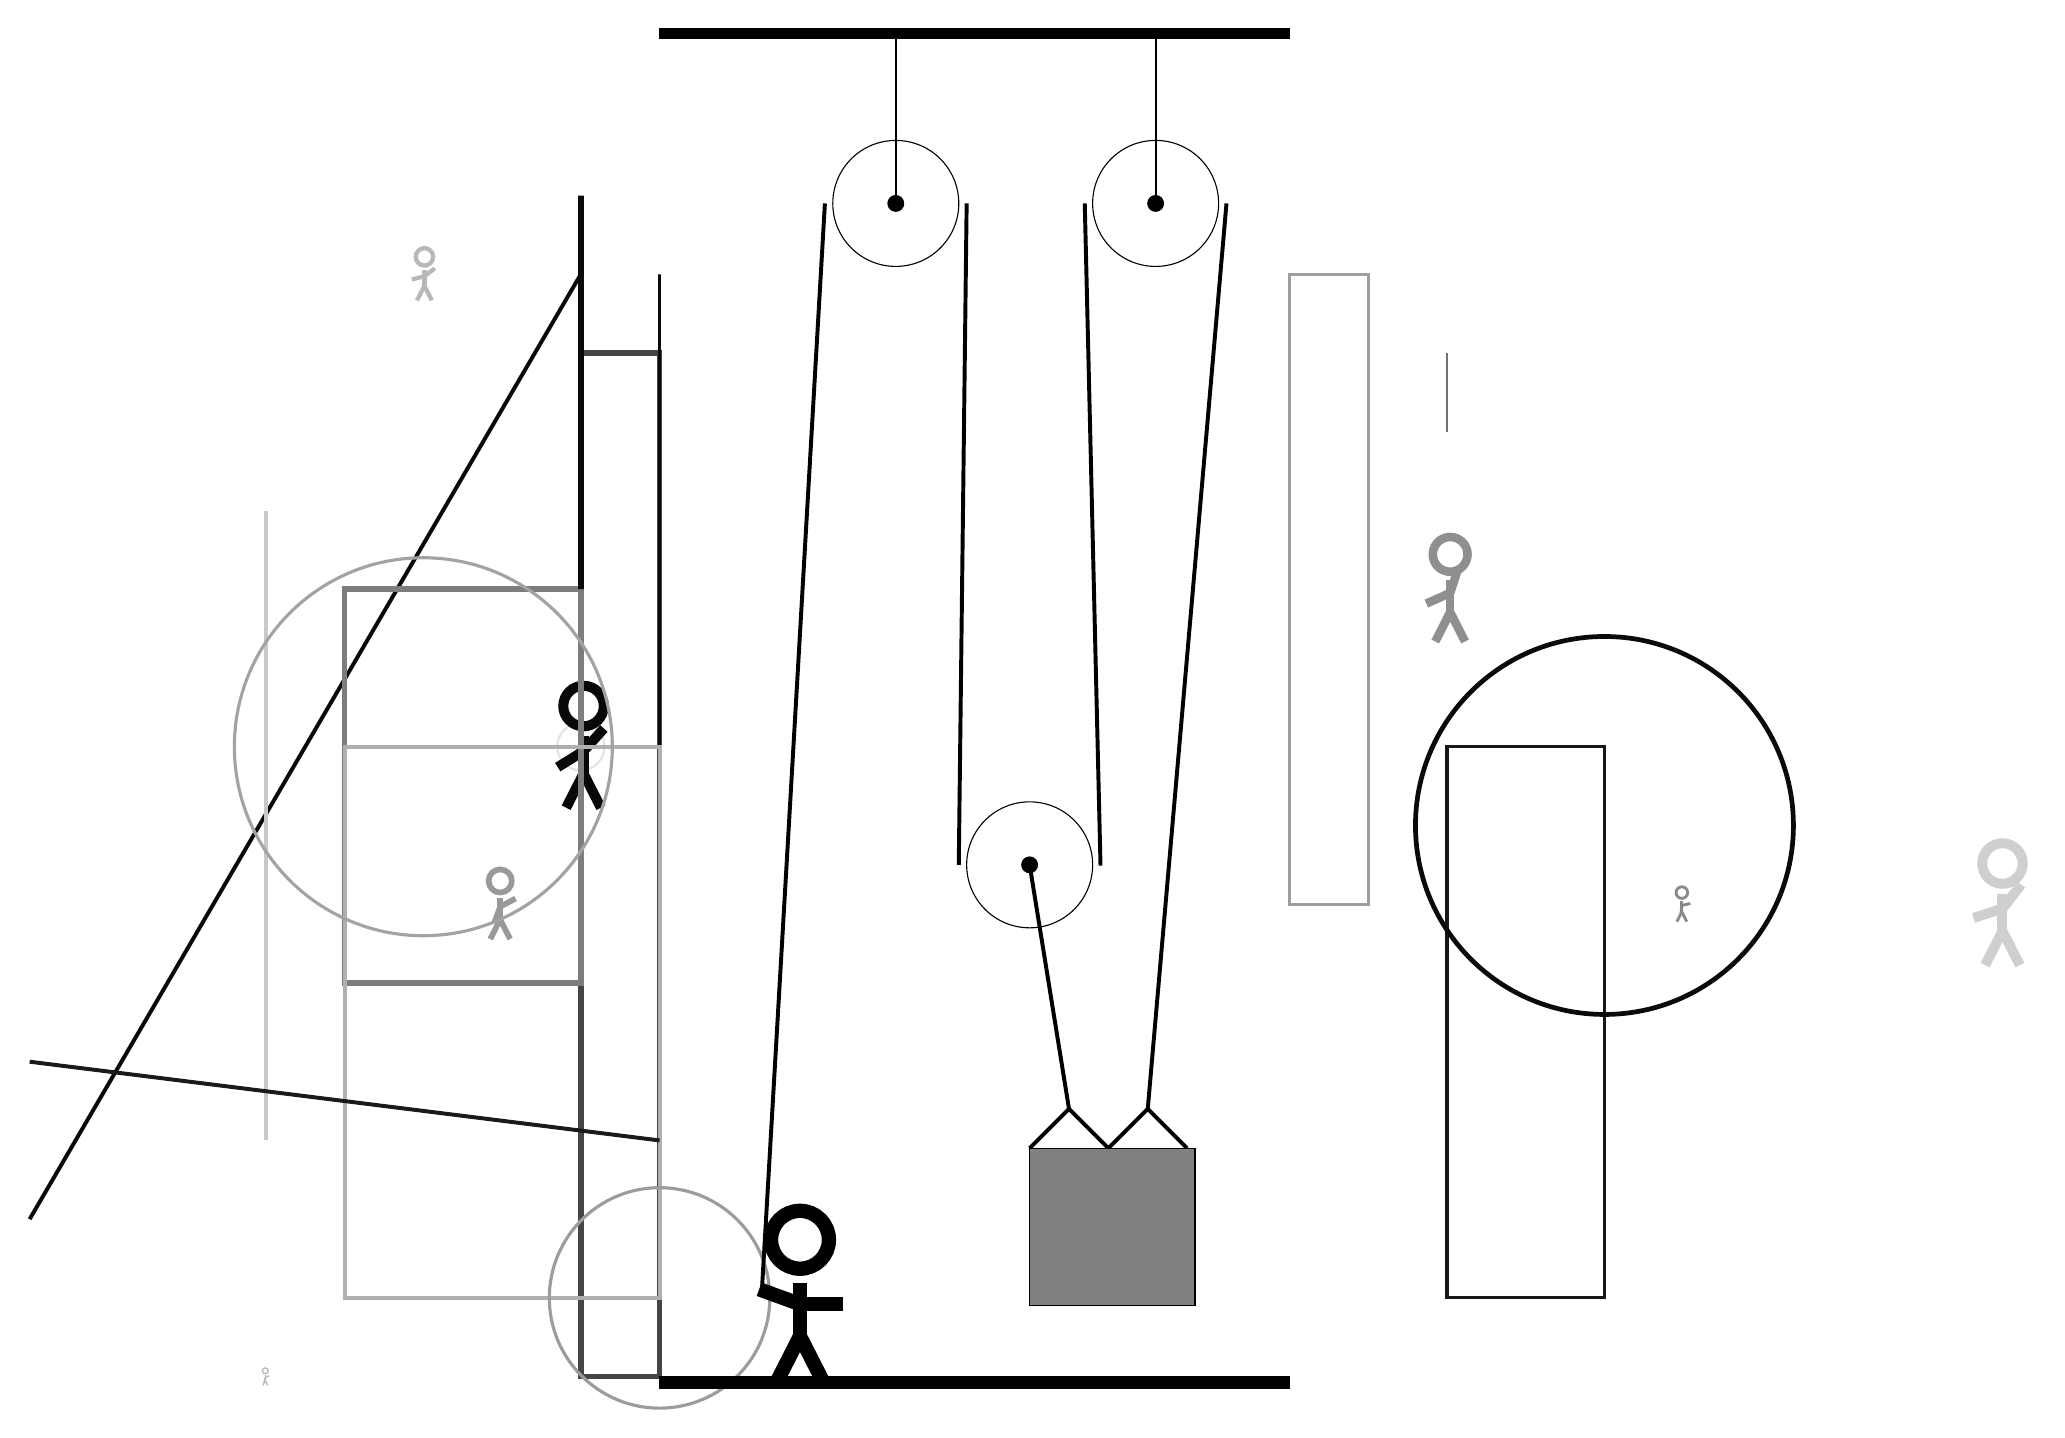
\begin{tikzpicture}
			%%%%% START %%%%%
			
			\draw[fill=black] (-2, 14) rectangle (6, 14.125);
			
			\draw [line width=0.3mm, color=black!10](-3, 5) circle (0.3);
			
			\node[line width=0.6mm, color=black!19] at (15, 3) {\Strichmaxerl[7][18][52]};
			\node[line width=0.4mm, color=black!28] at (-5, 11) {\Strichmaxerl[3][15][37]};
			\draw[line width=0.5mm, color=black!96](-3, 11) -- (-10, -1);
			\node[line width=0.4mm, color=black!46] at (11, 3) {\Strichmaxerl[2][84][13]};
			
			\draw[line width=0.4mm, color=black!38] (7, 11) rectangle (6, 3);
			\draw[line width=0.7mm, color=black!73] (-2, -3) rectangle (-3, 10);
			\node[line width=0.2mm, color=black!97] at (-3, 5) {\Strichmaxerl[7][32][48]};
			\node[line width=0.6mm, color=black!27] at (-7, -3) {\Strichmaxerl[1][74][20]};
			
			\draw[line width=0.4mm, color=black!91] (8, 5) rectangle (10, -2);
			
			\draw[line width=0.7mm, color=black!51] (-3, 7) rectangle (-6, 2);
			\node[line width=0.4mm, color=black!44] at (8, 7) {\Strichmaxerl[6][24][72]};
			\draw[line width=0.4mm, color=black!96] (-2, 11) rectangle (-2, 5);
			
			\node[line width=0.4mm, color=black!40] at (-4, 3) {\Strichmaxerl[4][70][28]};
			\draw[line width=0.5mm, color=black!21](-7, 0) -- (-7, 8);
			\draw[line width=0.5mm, color=black!31] (-2, 5) rectangle (-6, -2);
			
			\draw [line width=0.4mm, color=black!39](-2, -2) circle (1.4);
			
			\draw[line width=0.5mm, color=black!90](-2, 0) -- (-10, 1);
			\draw[line width=0.7mm, color=black!96] (-3, 7) rectangle (-3, 12);
			
			\draw[line width=0.3mm, color=black!55] (8, 9) rectangle (8, 10);
			\draw [line width=0.4mm, color=black!36](-5, 5) circle (2.4);
			
			\draw [line width=0.6mm, color=black!96](10, 4) circle (2.4);
			\draw[line width=0.4mm, color=black!79] (6, 7) rectangle (6, 7);
			
			\draw (1, 11.9) circle (0.8);
			\draw[fill=black] (1, 11.9) circle (0.1);
			\draw[thick] (1, 11.9) -- (1, 14);
			
			\draw (4.3, 11.9) circle (0.8);
			\draw[fill=black] (4.3, 11.9) circle (0.1);
			\draw[thick] (4.3, 11.9) -- (4.3, 14);
			
			\draw (2.7, 3.5) circle (0.8);
			\draw[fill=black] (2.7, 3.5) circle (0.1);
			
			\draw[line width=0.5mm]  (2.7, -0.1) -- (3.2, 0.4) -- (3.7, -0.1) -- (4.2, 0.4) -- (4.7, -0.1);
			\draw[fill=black!50] (2.7, -0.1) rectangle (4.8, -2.1);
			
			\draw[line width=0.5mm](-0.7, -1.9) -- (0.1, 11.9);
			\centerarc[line width=0.5mm](1, 11.9)(0:180:0.9);
			\draw[line width=0.5mm](1.9, 11.9) -- (1.8, 3.5);
			\centerarc[line width=0.5mm](2.7, 3.5)(180:370:0.9);
			\draw[line width=0.5mm] (3.6, 3.49) -- (3.4, 11.9);
			\centerarc[line width=0.5mm](4.3, 11.9)(0:180:0.9);
			\draw[line width=0.5mm](4.2, 0.4) -- (5.2, 11.9);
			\draw[line width=0.5mm] (3.2, 0.4) -- (2.7, 3.5);
			
			\node at (-0.2, -2) {\Strichmaxerl[10][-20][0]};
			
			\draw[fill=black] (-2, -3) rectangle (6, -3.15);
			
			%%%%% END %%%%%
		\end{tikzpicture}
	\end{figure}	
\end{document}